\documentclass[11pt]{article}

\usepackage[margin=1in]{geometry}
\usepackage{amsmath,amssymb}
\usepackage{booktabs}
\usepackage{graphicx}
\usepackage[round]{natbib}
\usepackage[hidelinks]{hyperref}

\renewcommand{\thefigure}{S\arabic{figure}}
\renewcommand{\thetable}{S\arabic{table}}
\renewcommand{\theequation}{S\arabic{equation}}

\title{Supplementary Material\\
Estimand Alignment in a Four-Arm Within-Study Comparison}
\author{Hanqing Yang}
\date{}

\begin{document}
\maketitle

\noindent
This supplement records exact numerical values, estimator formulas, and exploratory displays for the accompanying article. The prespecified primary interval is the one in the article's Table~2. Intervals computed by the later four-cell bootstrap, and intervals computed from 1{,}000-replicate trimming runs, are labeled as such wherever they appear. Machine-precision values below are the audited estimates. Rounded values in the article are the corresponding three-decimal, or, for the primary difference, five-decimal, displays.

\section{Exact primary and full-sample estimates}
\label{sec:exact}

Table~\ref{tab:exact-primary} restates the prespecified primary comparison without rounding. The contrast interval is the percentile interval from 2{,}000 successful replicates of the bootstrap that redraws G1, G2, and G4. The analytic standard errors are the two-sample standard error for the randomized difference in means and the cross-fit score standard error for the observational estimator.

\begin{table}[ht]
\centering
\caption{Unrounded prespecified primary estimates.}
\label{tab:exact-primary}
\small
\begin{tabular}{lr}
\toprule
Quantity & Value \\
\midrule
Randomized $\widehat\tau_1$ & 0.794681731104145 \\
Analytic SE & 0.2777657065981394 \\
Analytic interval & $[0.25027095003147215,\; 1.3390925121768178]$ \\
Observational ATT & 0.7942342079185714 \\
Score SE & 0.22379148303184127 \\
Analytic interval & $[0.35561096112935586,\; 1.2328574547077868]$ \\
Difference, observational minus randomized & $-0.00044752318557361725$ \\
Prespecified bootstrap SE & 0.4216686503551098 \\
Prespecified percentile interval & $[-0.9491600721638183,\; 0.6638487257328824]$ \\
Successful replicates & 2{,}000 of 2{,}000 \\
\bottomrule
\end{tabular}
\end{table}

Table~\ref{tab:exact-secondary} records the earlier full-sample contrast. The observational point estimate differs from the later independent evaluation 1.0753974159386461 by about $3\times 10^{-15}$. The percentile interval in this table is the one attached to the earlier contrast. It is not the interval for $\widehat\tau^{\mathrm{QED}}_{\mathrm{ATE}}-\widehat\tau_C$.

\begin{table}[ht]
\centering
\caption{Unrounded full-sample contrast from the earlier secondary analysis.}
\label{tab:exact-secondary}
\small
\begin{tabular}{lr}
\toprule
Quantity & Value \\
\midrule
Full-sample randomized difference in means & 0.7603449645239859 \\
Analytic SE & 0.1510881033486582 \\
Analytic interval & $[0.4642177234681503,\; 1.0564722055798215]$ \\
Observational ATE & 1.0753974159386432 \\
Score SE & 0.23320145971183331 \\
Analytic interval & $[0.6183309537612816,\; 1.532463878116005]$ \\
Difference & 0.3150524514146573 \\
Bootstrap SE & 0.45778170858020434 \\
Percentile interval & $[-0.6249039850074877,\; 1.1444295170363872]$ \\
Successful replicates & 2{,}000 of 2{,}000 \\
\bottomrule
\end{tabular}
\end{table}

The audited decomposition uses the concordant benchmark $\widehat\tau_C=0.7871551881338373$, the post-stratified benchmark $\widehat\tau_{\mathrm{ps}}=0.7873106895098261$, and the three components 0.2882422278048088, $-0.00015550137598874247$, and 0.026965724985840156. Their sum equals the unrounded full-sample discrepancy from the independent evaluation, 0.3150524514146602. The largest absolute row-wise identity error in the 2{,}000 four-cell replicates is $4.4\times 10^{-16}$.

The composition interval is $[-0.009506190156394149,\; 0.009796262064525704]$. The weight $\widehat\pi_c-\widehat\pi$ equals $-0.015275606746194936$ in every replicate. The resulting conditional interval for $\widehat\tau_1-\widehat\tau_0$ is approximately $[-0.641,\; 0.622]$. The point estimate is $0.010179718460452847$. The interval for the post-stratified minus unadjusted randomized term, also conditional on the cell sizes, is $[0.023764395892533707,\; 0.03006175914015258]$.

\section{Cross-fit scores and the second bootstrap}
\label{sec:scores}

On an estimation sample of size $n$, let $D_i$ be the treatment indicator, $Y_i$ the observed outcome, $e_i$ the out-of-fold propensity score, and $(\mu_{1i},\mu_{0i})$ the out-of-fold arm-specific outcome predictions. Clipping replaces $e_i$ by its projection onto $[10^{-6},\,1-10^{-6}]$. For the average treatment effect the cross-fit score of \citet{bang2005} is
\begin{equation}
(\mu_{1i}-\mu_{0i})
+
\frac{D_i}{e_i}(Y_i-\mu_{1i})
-
\frac{1-D_i}{1-e_i}(Y_i-\mu_{0i}).
\label{eq:ate-score}
\end{equation}
For the average treatment effect on the treated, with $p$ held at the mean of $D$ in the estimation sample,
\begin{equation}
\frac{D_i}{p}(Y_i-\mu_{0i})
-
\frac{(1-D_i)\,e_i}{p\,(1-e_i)}(Y_i-\mu_{0i}).
\label{eq:att-score}
\end{equation}
The untreated score is the treated score after the treatment labels are reversed. Folds are ordinary $K$-fold partitions with $K=5$, not stratified folds. In the prespecified fit the random seed is 20261026. The reported analytic standard error uses the raw scores, with divisor $n-1$ inside the standard deviation. A recentered influence function that treats $p$ as estimated is a different standard error; it was not the primary reported standard error, and it is not the bootstrap standard deviation.

The independent implementation reproduced the primary observational point estimate to within $1.3\times 10^{-15}$ and the primary randomized estimate exactly. Its four-cell bootstrap is summarized in Table~\ref{tab:impl}. The contrast standard deviation is about 0.470, and the percentile interval is about $[-0.925,\,0.661]$. This bootstrap redraws G1, G2, G3, and G4, whereas the prespecified bootstrap redraws only G1, G2, and G4. The random-number streams also differ, and the observational treated-effect margin has a heavy tail. The interval is an implementation-specific sensitivity result. Table~\ref{tab:exact-primary} is unchanged by it.

In that margin, 41 replicates of the observational treated estimate are negative and one is below $-2$. The minimum is about $-8.62$, and the excess kurtosis is 163.25. The percentile interval is sensitive to this tail. Dividing the interquartile range by 1.349 gives 0.307, which describes the center of the distribution only. The untreated and average-effect margins do not have a comparable single-replicate spike; their excess kurtosis is about 4.

\begin{table}[ht]
\centering
\caption{Four-cell bootstrap quantities from the independent implementation. These values do not replace Table~\ref{tab:exact-primary}.}
\label{tab:impl}
\small
\begin{tabular}{lr}
\toprule
Quantity & Value \\
\midrule
Primary-contrast bootstrap SD & 0.4704077152493183 \\
Primary-contrast 2.5th percentile & $-0.9251154466640124$ \\
Primary-contrast 97.5th percentile & 0.6610285346256077 \\
Observational ATT bootstrap SD & 0.38874647117306493 \\
Observational ATT 2.5th percentile & 0.03410392205623919 \\
Observational ATT 97.5th percentile & 1.346552534607815 \\
Minimum observational ATT & $-8.621320612422295$ \\
\bottomrule
\end{tabular}
\end{table}

Figure~\ref{fig:aligned} plots, for each scalar, the point estimate and the 2.5th and 97.5th percentiles from this same four-cell file. The three pairs are the treated contrast against $\widehat\tau_1$, the untreated contrast against $\widehat\tau_0$, and the average-effect contrast against $\widehat\tau_C$. Each bar is a marginal percentile interval. The figure does not display the prespecified analytic intervals, it does not display the prespecified primary contrast interval, and the three intervals are not a simultaneous band. The axis text generated with the figure describes the intervals as joint-bootstrap percentile intervals. The jointness of the redraw means that the estimates in one row share a sample. The plotted endpoints remain marginal.

\begin{figure}[ht]
\centering
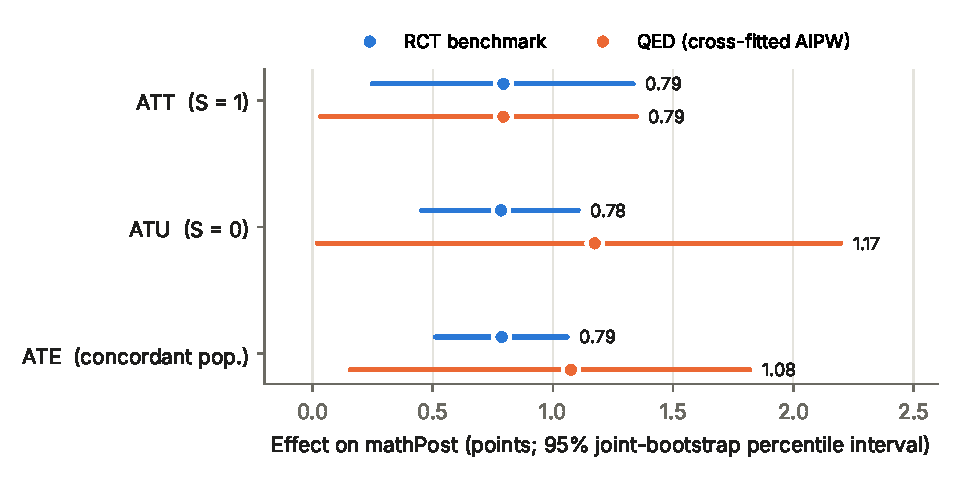
\includegraphics[width=0.92\textwidth]{figures/fig1_aligned_estimates.pdf}
\caption{Point estimates and marginal 95\% percentile intervals from the four-cell bootstrap. Blue denotes the randomized benchmark and orange the cross-fit observational estimator. The treated observational interval is affected by a replicate near $-8.62$. These intervals do not replace the prespecified primary interval.}
\label{fig:aligned}
\end{figure}

The numerical reproduction of the point estimates and of the saved bootstrap summaries was obtained with Python~3.12.10 and scikit-learn~1.6.1. A written note accompanying the reanalysis names Python~3.13 and scikit-learn~1.9. The estimates still matched to at most $2.8\times 10^{-14}$ across the saved point estimates, bootstrap summaries, seed file, covariate file, sensitivity bounds, and trimming table. That match is a match of estimands and numbers. It is not a reconstruction of the original execution process.

\section{Cross-fitting seeds}
\label{sec:seeds}

Figure~\ref{fig:seeds} and Table~\ref{tab:seeds} summarize 200 fold seeds on the fixed sample. The median observational treated estimate is 0.7338163919022771. The prespecified seed's treated estimate is at the 77th percentile of these 200 numbers, and 11.5 percent of the seeds yield an absolute contrast with $\widehat\tau_1$ below 0.01. The dashed line in the figure marks that prespecified seed. The solid line marks the randomized benchmark.

\begin{table}[ht]
\centering
\caption{Observational estimates across 200 fold seeds.}
\label{tab:seeds}
\begin{tabular}{lrrr}
\toprule
 & ATT & ATU & ATE \\
\midrule
Median & 0.734 & 1.196 & 1.076 \\
5th percentile & 0.641 & 1.014 & 0.942 \\
95th percentile & 0.833 & 1.368 & 1.195 \\
Minimum & 0.580 & 0.548 & 0.609 \\
Maximum & 0.865 & 1.453 & 1.283 \\
Standard deviation & 0.061 & 0.116 & 0.088 \\
\bottomrule
\end{tabular}
\end{table}

\begin{figure}[ht]
\centering
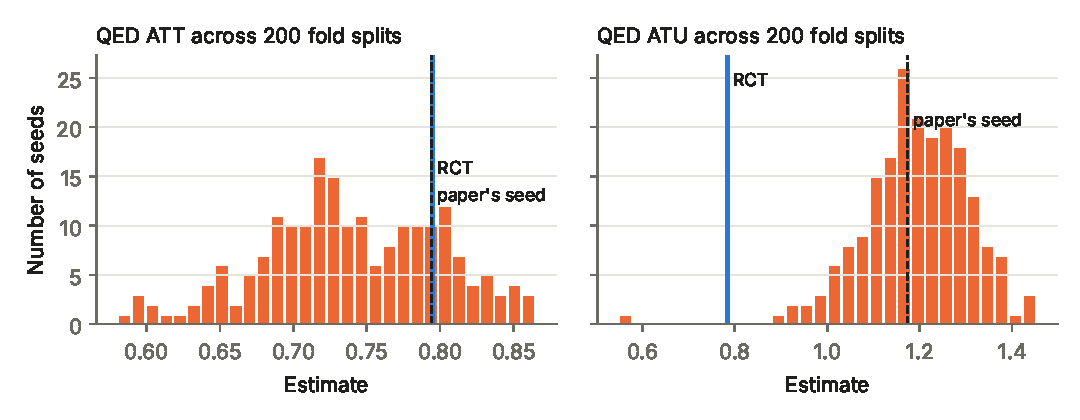
\includegraphics[width=0.92\textwidth]{figures/fig2_fold_seeds.pdf}
\caption{Histograms of the observational treated and untreated estimates over 200 fold seeds. The seeds repartition one sample. They are not replications of the study.}
\label{fig:seeds}
\end{figure}

\section{Covariate sets}
\label{sec:covs}

The nested sets in Table~\ref{tab:nested} and Figure~\ref{fig:covs} add, in order, eleven demographic and schooling variables, the mathematics and vocabulary pre-tests, four mathematics-motivation measures (\texttt{mathLike}, \texttt{calc}, \texttt{AMAS}, \texttt{MCS}), and eight personality and related scales, including \texttt{logBooks}. Each nonempty entry is a median over seeds 1 through 50. The empty entry is one concordant difference in means, copied into all three columns. Discrepancies subtract $\widehat\tau_1$, $\widehat\tau_0$, and $\widehat\tau_C$ respectively. The full-set median treated estimate, 0.738, is not the prespecified estimate 0.794.

\begin{table}[ht]
\centering
\caption{Median observational estimates and discrepancies by covariate set.}
\label{tab:nested}
\begin{tabular}{lrrrrrr}
\toprule
Set & ATT & ATU & ATE & $\Delta$ATT & $\Delta$ATU & $\Delta$ATE \\
\midrule
None & 3.451 & 3.451 & 3.451 & 2.656 & 2.666 & 2.663 \\
Demographics & 2.952 & 3.143 & 3.094 & 2.157 & 2.359 & 2.307 \\
Plus pre-tests & 1.594 & 1.747 & 1.707 & 0.799 & 0.962 & 0.920 \\
Plus motivation & 0.735 & 1.174 & 1.066 & $-0.060$ & 0.389 & 0.279 \\
Full set & 0.738 & 1.209 & 1.091 & $-0.056$ & 0.425 & 0.304 \\
\bottomrule
\end{tabular}
\end{table}

\begin{figure}[ht]
\centering
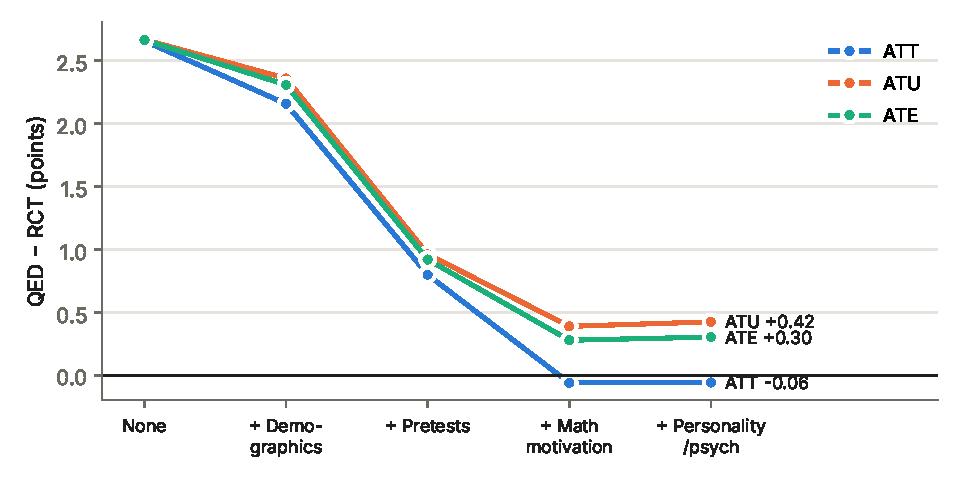
\includegraphics[width=0.85\textwidth]{figures/fig3_covariate_sets.pdf}
\caption{Discrepancies from the randomized benchmarks as covariates are added. The empty-set discrepancies differ across estimands only because the benchmarks differ. The paths are exploratory medians over 50 seeds.}
\label{fig:covs}
\end{figure}

Table~\ref{tab:loo} reports the largest median leave-one-out shifts relative to the full-set median. A positive shift means that omitting the named covariate raises the median observational estimate. Omitting \texttt{mathPre} shifts the treated median by 0.669 and the untreated median by 0.235. Omitting \texttt{mathLike} shifts the treated median by 0.249 and the untreated median by 0.011. These quantities are not an additive decomposition of selection bias.

\begin{table}[ht]
\centering
\caption{Largest median leave-one-out shifts relative to the full covariate set.}
\label{tab:loo}
\begin{tabular}{lrrr}
\toprule
Omitted covariate & Treated shift & Untreated shift & ATE shift \\
\midrule
\texttt{mathPre} & 0.669 & 0.235 & 0.340 \\
\texttt{mathLike} & 0.249 & 0.011 & 0.072 \\
\texttt{MCS} & 0.179 & 0.089 & 0.107 \\
\texttt{AMAS} & 0.037 & 0.189 & 0.146 \\
\texttt{vocabPre} & $-0.115$ & $-0.118$ & $-0.117$ \\
\texttt{big5A} & 0.002 & $-0.101$ & $-0.065$ \\
\bottomrule
\end{tabular}
\end{table}

After weighting, the largest absolute standardized difference in the primary treated comparison is 0.143, on the vocabulary pre-test. Three covariates exceed 0.1 in absolute value, and none exceeds 0.2. In the untreated weighting, the largest absolute standardized difference is 0.292, on agreeableness (\texttt{big5A}), and four covariates exceed 0.1. The treated-comparison effective sample size is 145.918 of 817, the maximum control weight is 7.703, and the ten largest control weights account for 19.1 percent of the weight. The untreated-comparison figures are an effective sample size of 61.929 of 288, a maximum weight of 52.572, and a top-ten share of 31.3 percent.

\section{Sensitivity grid}
\label{sec:sens}

Table~\ref{tab:sens} and Figure~\ref{fig:sens} report the inverse-probability bounds. The column ``RCT inside the point bounds'' refers to the numerical bounds at that $\Lambda$, not to the percentile interval of the endpoints. At $\Lambda=1$ the point bounds collapse to the H{\'a}jek estimates 0.6857768855171429 and 0.9596311794657346 and do not contain the randomized points. The endpoint intervals at $\Lambda=1$ do extend below those randomized points. The augmented untreated estimate, 1.1745100278233231, exceeds the inverse-probability value by 0.2148788483575885. The grid value $\Lambda=1.06$ is not a row of Table~\ref{tab:sens}; it is the first point, on a separate grid with step 0.01, at which the untreated lower point bound is at most $\widehat\tau_0$.

\begin{table}[ht]
\centering
\caption{Inverse-probability sensitivity bounds. Endpoint intervals are percentile intervals of the bound endpoints from 1{,}000 replicates.}
\label{tab:sens}
\small
\begin{tabular}{llrrrrc}
\toprule
$\Lambda$ & Estimand & Lower & Upper & Endpoint low & Endpoint high & RCT in bounds \\
\midrule
1.00 & ATT & 0.686 & 0.686 & $-0.252$ & 1.287 & No \\
1.00 & ATU & 0.960 & 0.960 & $-0.340$ & 2.007 & No \\
1.10 & ATT & 0.395 & 0.983 & $-0.534$ & 1.590 & Yes \\
1.10 & ATU & 0.662 & 1.258 & $-0.612$ & 2.291 & Yes \\
1.25 & ATT & 0.016 & 1.385 & $-0.887$ & 1.992 & Yes \\
1.25 & ATU & 0.272 & 1.657 & $-0.994$ & 2.637 & Yes \\
1.50 & ATT & $-0.496$ & 1.968 & $-1.365$ & 2.565 & Yes \\
1.50 & ATU & $-0.286$ & 2.203 & $-1.515$ & 3.140 & Yes \\
1.75 & ATT & $-0.897$ & 2.455 & $-1.712$ & 3.027 & Yes \\
1.75 & ATU & $-0.735$ & 2.676 & $-1.957$ & 3.601 & Yes \\
2.00 & ATT & $-1.227$ & 2.876 & $-1.999$ & 3.435 & Yes \\
2.00 & ATU & $-1.128$ & 3.061 & $-2.282$ & 3.936 & Yes \\
2.50 & ATT & $-1.696$ & 3.542 & $-2.432$ & 4.088 & Yes \\
2.50 & ATU & $-1.736$ & 3.697 & $-2.824$ & 4.462 & Yes \\
3.00 & ATT & $-2.051$ & 4.051 & $-2.706$ & 4.578 & Yes \\
3.00 & ATU & $-2.197$ & 4.154 & $-3.297$ & 4.854 & Yes \\
\bottomrule
\end{tabular}
\end{table}

\begin{figure}[ht]
\centering
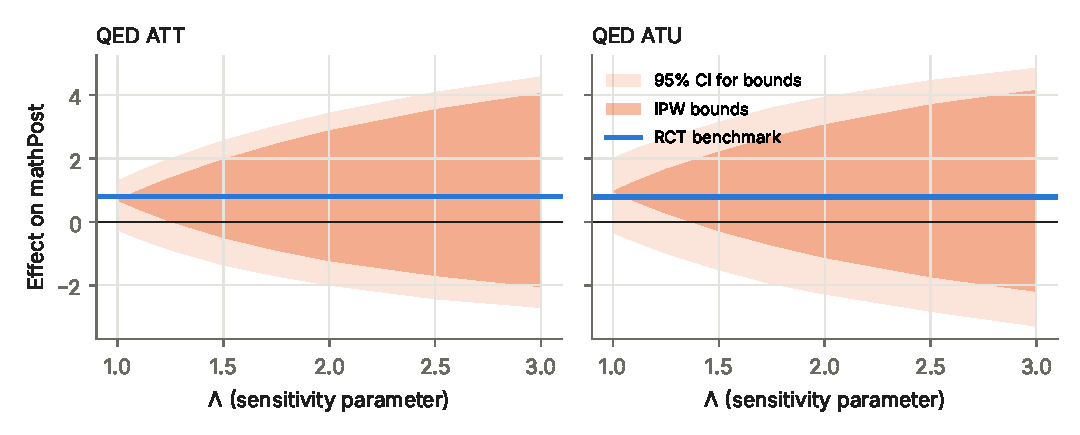
\includegraphics[width=0.92\textwidth]{figures/fig4_sensitivity.pdf}
\caption{Point bounds and endpoint percentile bands for the inverse-probability functionals, with the randomized benchmark drawn in blue. The darker band is the point-bound interval. The lighter band is not a confidence interval for the causal effect. The bounds are not sharp bounds for inverse-probability weighting, and they do not apply to the augmented estimator.}
\label{fig:sens}
\end{figure}

\section{Trimming}
\label{sec:trim}

Table~\ref{tab:trim} reports regions defined by a propensity score fit on the concordant covariates, without the outcome, and then held fixed for the full sample of 2{,}200. The bootstrap redraws within the region and does not refit the trimming score. Every row is a different target population. The interval in the untrimmed row comes from 1{,}000 replicates and is not a primary or a 2{,}000-replicate interval. The Crump threshold fit on the concordant sample is $\alpha=0.084311327831958$, reported in the table as 0.084.

\begin{table}[ht]
\centering
\caption{Exploratory overlap regions. Sample sizes for G1 and G4 are the concordant cells inside the region. Intervals are percentile intervals from the trimming bootstrap.}
\label{tab:trim}
\small
\begin{tabular}{lrrrrrr}
\toprule
Region & $n$ & G1 / G4 & $\widehat\tau_0$ & $\Delta$ATT & $\Delta$ATU & $\Delta$ATE \\
\midrule
Untrimmed & 2{,}200 & 288 / 817 & 0.785 & $-0.000$ & 0.390 & 0.288 \\
 & & & & $[-1.004,\,0.682]$ & $[-0.729,\,1.427]$ & $[-0.595,\,1.088]$ \\
$[0.05,\,0.95]$ & 1{,}846 & 281 / 624 & 0.503 & 0.120 & 0.422 & 0.328 \\
 & & & & $[-0.891,\,0.781]$ & $[-0.483,\,1.994]$ & $[-0.349,\,1.368]$ \\
$[0.1,\,0.9]$ & 1{,}446 & 259 / 447 & 0.430 & $-0.231$ & 0.716 & 0.369 \\
 & & & & $[-1.276,\,0.722]$ & $[-0.918,\,2.317]$ & $[-0.697,\,1.399]$ \\
Crump, $\alpha=0.084$ & 1{,}561 & 268 / 495 & 0.404 & $-0.011$ & 0.640 & 0.411 \\
 & & & & $[-1.008,\,0.714]$ & $[-1.033,\,2.209]$ & $[-0.715,\,1.449]$ \\
\bottomrule
\end{tabular}
\end{table}

\bibliographystyle{apalike}
\bibliography{references}

\end{document}
